\documentclass[conference,compsoc]{IEEEtran}
\IEEEoverridecommandlockouts
% The preceding line is only needed to identify funding in the first footnote. If that is unneeded, please comment it out.

\usepackage{cite,doi}
\usepackage{amsmath,amssymb,amsfonts}
\usepackage{algorithm,algpseudocode}
\usepackage{graphicx}
\usepackage{textcomp}
\usepackage{xcolor}
\usepackage{cleveref}
\usepackage{tikz}
\usepackage{ourmacros}
\def\BibTeX{{\rm B\kern-.05em{\sc i\kern-.025em b}\kern-.08em
    T\kern-.1667em\lower.7ex\hbox{E}\kern-.125emX}}

\newcommand{\LM}[1]{\textcolor{blue}{\textbf{Lawton}: #1}}    
\newcommand{\GB}[1]{\textcolor{red}{\textbf{Grey}: #1}}
\newcommand{\RK}[1]{\textcolor{blue}{\textbf{Ramki}: #1}}


\begin{document}

\title{Parallel Hierarchical Clustering using \\ Rank-Two Nonnegative Matrix Factorization
\thanks{This material is based upon work supported by the National Science Foundation under Grant No. OAC-1642385 and OAC-1642410.
This manuscript has been co-authored by UT-Battelle, LLC under Contract No. DE-AC05-00OR22725 with the U.S. Department of
Energy. This project was partially funded by the Laboratory Director's Research and Development fund. This research used resources
of the Oak Ridge Leadership Computing Facility at the Oak Ridge National Laboratory, which is supported by the Office of Science of
the U.S. Department of Energy.}
}

\author{\IEEEauthorblockN{Lawton Manning and Grey Ballard}
\IEEEauthorblockA{Wake Forest University \\
Winston-Salem, NC, USA \\
\{mannlg15,ballard\}@wfu.edu}
\and
\IEEEauthorblockN{Ramakrishnan Kannan}
\IEEEauthorblockA{Oak Ridge National Laboratory \\
Oak Ridge, TN, USA \\
kannanr@ornl.gov}
\and
\IEEEauthorblockN{Haesun Park}
\IEEEauthorblockA{Georgia Institute of Technology \\
Atlanta, GA, USA \\
hpark@cc.gatech.edu}
}

\maketitle

\begin{abstract}
Nonnegative Matrix Factorization (NMF) is an effective tool for clustering nonnegative data, either for computing a flat partitioning of a dataset or for determining a hierarchy of similarity.
In this paper, we propose a parallel algorithm for hierarchical clustering that uses a divide-and-conquer approach based on rank-two NMF to split a data set into two cohesive parts.
Not only does this approach uncover more structure in the data than a flat NMF clustering, but also rank-two NMF can be computed more quickly than for general ranks, providing comparable overall time to solution.
Furthermore, the rank-two NMF algorithm can be parallelized efficiently using a computational kernel similar to matrix-vector multiplication.
Our data distribution and parallelization strategies are designed to maintain computational load balance throughout the data-dependent hierarchy of computation while limiting interprocess communication, allowing the algorithm to scale to large dense and sparse data sets.
We demonstrate the scalability of our parallel algorithm in terms of data size and number of processors, and apply the hierarchical clustering approach to large (dense) hyperspectral imaging and (sparse) text document data.
\end{abstract}

%\begin{IEEEkeywords}
%component, formatting, style, styling, insert
%\end{IEEEkeywords}

\section{Introduction}

\GB{ask Haesun to write intro paragraph motivating hierarchical clustering but noting the limitations of time and data size?}

\section{Preliminaries}

\begin{itemize}
	\item NMF, BCD, rank-2 NMF
	\item PLANC
\end{itemize}

\section{Algorithm}

\subsection{Sequential Algorithm}

\subsubsection{Rank-2 NMF}

\begin{algorithm}
\caption{Rank-2 Nonnegative Least Squares Solve \cite{KP13}}
\label{alg:r2nmf}
\begin{algorithmic}[1]
	\Require{$\M{C}$ is $n\times 2$ and $\M{G}$ is $2\times 2$ and s.p.d.}
	\Function{$\M{H} =$ Rank2-NLS-Solve}{$\M{C},\M{G}$}
		\State $\M{H} = \M{C}\M{G}^{-1}$
		\For{$i=1$ to $n$}
			\If{$\ME{H}{i1} < 0$ or $\ME{H}{i2} < 0$}
				\If{$\ME{H}{i1} \sqrt{\ME{G}{11}}  < \ME{H}{i2} \sqrt{\ME{G}{22}} $}
					\State $\ME{H}{i1} = 0$
					\State $\ME{H}{i2} = \ME{C}{i2} / \ME{G}{22}$
				\Else
					\State $\ME{H}{i1} = \ME{C}{i1} / \ME{G}{11}$
					\State $\ME{H}{i2} = 0$
				\EndIf
			\EndIf
		\EndFor
	\EndFunction
	\Ensure{$\displaystyle \M{H} = \argmin_{\M[\bar]{H} \geq \M{0}} \|\M{A}-\M{W}\M[\bar]{H}^\Tra\|$ is $n\times 2$ with $\M{C}=\M{A}^\Tra \M{W}$ and $\M{G}=\M{W}^\Tra\M{W}$}
\end{algorithmic}
\end{algorithm}

\subsubsection{Hierarchical Clustering}

\begin{algorithm}
\caption{Hierarchical Clustering \cite{KP13}}
\label{alg:hiernmf2}
\begin{algorithmic}[1]
	\Require{$\M{A}$ is $m\times n$, $k$ is target number of leaves}
	\Function{${\cal T} =$ Hier-R2-NMF}{$\M{A}$}
		\State ${\cal R} = \text{node}(\M{A})$ \hfill \Comment{create root node}
		\State \textsc{Split}$({\cal R})$
		\State inject$({\cal Q},{\cal R}.\text{left})$ \hfill \Comment{create priority queue}
		\State inject$({\cal Q},{\cal R}.\text{right})$ \hfill \Comment{of frontier nodes}
		\While{size$({\cal Q}) < k$}
			\State ${\cal N} = \text{eject}({\cal Q})$ \hfill \Comment{get leaf with max score}
			\State \textsc{Split}$({\cal R}.\text{left})$ \hfill \Comment{split left child}
			\State inject$({\cal Q},{\cal R}.\text{left})$ \hfill \Comment{and add to $\cal Q$}
			\State \textsc{Split}$({\cal R}.\text{right})$ \hfill \Comment{split right child}
			\State inject$({\cal Q},{\cal R}.\text{right})$ \hfill \Comment{and add to $\cal Q$}
		\EndWhile
	\EndFunction
	\Ensure{$\cal{T}$ is binary tree rooted at $\cal R$ with $k$ frontier nodes, each node has subset of cols of $\M{A}$ and feature vector $\V{w}$}
\end{algorithmic}
\end{algorithm}

\begin{figure}
%!TEX root = ../paper.tex

\centering
\scalebox{.7}{
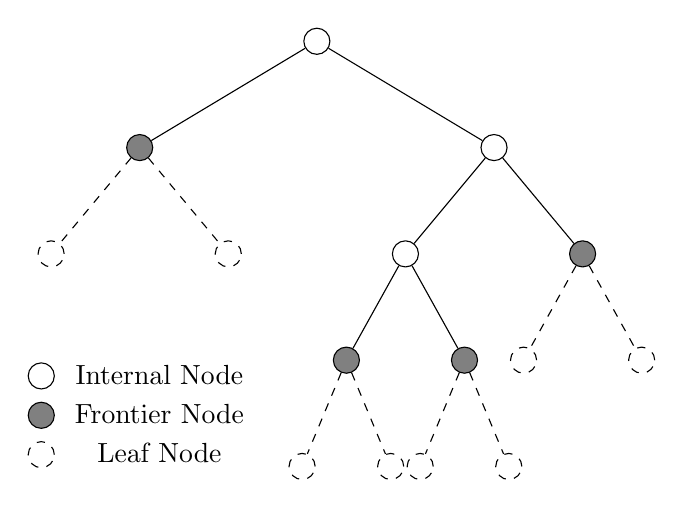
\begin{tikzpicture}[scale=.9,level/.style={sibling distance=50mm/#1}]
\node [circle,draw] (z) {}
  child {node [circle,draw,fill=gray] (a) {}
    child[dashed] {node [circle,draw,dashed] (b) {}}
    child[dashed] {node [circle,draw,dashed] (g) {}}
  }
  child {node [circle,draw] (j) {}
    child {node [circle,draw] (k) {}
      child {node [circle,draw,fill=gray] (o) {}
        child[dashed] {node [circle,draw,dashed] (x) {}}
        child[dashed] {node [circle,draw,dashed] (y) {}}
      }
      child {node [circle,draw,fill=gray] (p) {}
        child[dashed] {node [circle,draw,dashed] (x) {}}
        child[dashed] {node [circle,draw,dashed] (y) {}}
      }
    }
  child {node [circle,draw,fill=gray] (l) {}
    child[dashed] {node [circle,draw,dashed] (c) {}}
    child[dashed] {node [circle,draw,dashed] (d) {}}
  }
};

\node [shift={(-3.5,-4.25)},circle,draw,label={[xshift=1.5cm, yshift=-0.4cm] Internal Node}] (leg1) {};
\node [shift={(-3.5,-4.75)},circle,draw,fill=gray,label={[xshift=1.5cm, yshift=-0.4cm] Frontier Node}] (leg1) {};
\node [shift={(-3.5,-5.25)},circle,draw,dashed,label={[xshift=1.5cm, yshift=-0.4cm] Leaf Node}] (leg1) {};
\end{tikzpicture}
}
\caption{Hierarchy node classification}
\label{fig:tree}
\end{figure}

\begin{algorithm}
\caption{Node Splitting via Rank-Two NMF}
\label{alg:split}
\begin{algorithmic}[1]
	\Require{$\cal N$ has a subset of columns given by field $\M{A}$}
	\Function{Split}{$\cal N$}
		\State $[\M{W},\M{H}] = \textsc{Rank2-NMF}({\cal N}.\M{A})$ \hfill \Comment{split $\cal N$}
		\State partition ${\cal N}.\M{A}$ into $\M{A}_1$ and $\M{A}_2$ using $\M{H}$
		\State ${\cal N}.\text{left} = \text{node}(\M{A}_1,\V{W}_1)$ \hfill \Comment{create left child}
		\State ${\cal N}.\text{right} = \text{node}(\M{A}_2,\V{W}_2)$ \hfill \Comment{create right child}
		\State ${\cal N}.\text{score} = \sigma_1(\M{A}_1) + \sigma_1(\M{A}_2) - \sigma_1({\cal N}.\M{A})$
	\EndFunction
	\Ensure{$\cal{N}$ has two children and a score}
\end{algorithmic}
\end{algorithm}

\subsection{Parallelization}

\subsubsection{Algorithm}

\begin{algorithm}
\caption{Parallel Rank-2 NMF}
\label{alg:parrank2nmf}
\begin{algorithmic}[1]
	\Require{$\M{A}$ is $m\times n$ and row-distributed across processors so that $\M[\hat]{A}$ is local $(m/p)\times n$ submatrix}
	\Function{$[\M{W},\M{H}] =$ Parallel-Rank2-NMF}{$\M{A}$}
		\State Initialize local $\M[\hat]{W}$ randomly
		\While{not converged}
			\State \Comment{Compute $\M{H}$}
			\State $\M[\hat]{G}_W = \M[\hat]{W}^\Tra \M[\hat]{W}$
			\State $\M{G}_W = \textsc{All-Reduce}(\M[\hat]{G})$
			\State $\M[\hat]{B} = \M[\hat]{W}^\Tra \M[\hat]{A}$ %\hfill \Comment{local matrix multiplication}
			\State $\M[\hat]{C} = \textsc{Reduce-Scatter}(\M[\hat]{B})$
			\State $\M[\hat]{H} = \textsc{Rank2-NLS-Solve}(\M[\hat]{C},\M{G}_W)$
			\State \Comment{Compute $\M{W}$}
			\State $\M[\hat]{G}_H = \M[\hat]{H}^\Tra \M[\hat]{H}$
			\State $\M{G}_H = \textsc{All-Reduce}(\M[\hat]{G}_H)$
			\State $\M{H} = \textsc{All-Gather}(\M[\hat]{H})$
			\State $\M[\hat]{D} = \M[\hat]{A} \M{H}$ %\hfill \Comment{local matrix multiplication}
			\State $\M[\hat]{W} = \textsc{Rank2-NLS-Solve}(\M[\hat]{D},\M{G}_H)$
		\EndWhile
	\EndFunction
	\Ensure{$\M{A} \approx \M{W}\M{H}^\Tra$ with $\M{W}$, $\M{H}$ row-distributed}
\end{algorithmic}
\end{algorithm}

\begin{figure}
% !TEX root = ../paper.tex

\newcommand{\lightred}{red!75}
\newcommand{\lightblue}{blue!75}
\newcommand{\offset}{.1}

\begin{tikzpicture}

% draw A
\fill[\lightred] (0,0) rectangle ++(0.5,4);
\fill[\lightblue] (0.5,0) rectangle ++(1.25,4);
\fill[\lightred] (1.75,0) rectangle ++(1.25,4);
\fill[\lightblue] (3,0) rectangle ++(1,4);
\draw[thick,dashed,xscale=4,yscale=4/3] (0,0) grid ++(1,3);
\draw[thick] (0,0) rectangle (4,4);

% draw W
\draw[thick,shift={(-.5,0)},xscale=.15,yscale=4] (0,0) grid ++(2,1);

% draw H
\draw[thick,shift={(0,4.1)},xscale=4,yscale=.15] (0,) grid ++(1,2);]

\begin{scope}[shift={(-1,-6)}]
	% draw A_1 and w_1
	\draw[thick,fill=\lightred] (0,0) rectangle ++(2.25,4);
	\draw[thick,dashed,xscale=2.25,yscale=4/3] (0,0) grid ++(1,3);
	\draw[thick] (-.5,0) rectangle ++(.15,4);
	
	% draw A_2 and w_2
	\draw[thick,fill=\lightblue] (5,0) rectangle ++(1.75,4);
	\draw[thick,dashed,shift={(5,0)},xscale=1.75,yscale=4/3] (0,0) grid ++(1,3);
	\draw[thick,shift={(5,0)}] (-.5,0) rectangle ++(.15,4);
	
\end{scope}

% draw arrows to A_1 and w_1
% TODO: make these arrows prettier
\draw[thick] (0.25,-\offset) parabola (1.5,-0.5);
\draw[thick] (2.25,-\offset) parabola (1.5,-0.5);
\draw[thick,->] (1.5,-0.5) parabola (.125,-2+\offset);
\draw[thick,->] (-.5+.075,-\offset) parabola (-1.5+.075,-2+\offset);

% draw arrows to A_2
% TODO: make these arrows prettier
\draw[thick] (1,-\offset) parabola (2.5,-0.5);
\draw[thick] (3.5,-\offset) parabola (2.5,-0.5);
\draw[thick,->] (2.5,-0.5) parabola (4.875,-2+\offset);
\draw[thick,->] (-.5+.225,-\offset) parabola (3.5+.075,-2+\offset);

\end{tikzpicture}

\caption{Parallel splitting using Rank-2 NMF}
\label{fig:split}
\end{figure}

\subsubsection{Analysis}

\section{Experimental Results}

\subsection{Experimental Platform}

\GB{Lawton, can you add a description of Summit?  use the recent SC submission as an example}

\subsection{Datasets}

\GB{Lawton, can you add these descriptions?}
\begin{itemize}
	\item synthetic (dense and sparse)
	\item HSI: DC and Aviris
	\item Doc-clustering: Reuters and PubMed
\end{itemize}

\subsection{Performance}

\subsubsection{Rank-2 NMF Strong Scaling}

\GB{Lawton, can you gather this data, Ramki can you visualize it?}
\begin{itemize}
	\item compare 1D distribution scaling with optimal 2D grid scaling
	\item use synthetic short-and-fat dense and squarish sparse
\end{itemize}

\subsubsection{Level Scaling}

\GB{Ramki, can you add a bar plot to show time breakdown across complete levels?  Let's do Aviris and PubMed; just use levels data file}

\subsubsection{Weak Scaling}

\GB{maybe this section is lower priority}
\begin{itemize}
	\item dense and sparse
\end{itemize}

\subsubsection{Strong Scaling}

\begin{itemize}
	\item big dense synthetic
	\item big sparse synthetic
	\item Aviris
	\item PubMed
\end{itemize}

\subsection{Clustering}

\subsubsection{Hyperspectral Imaging}

\GB{Lawton, show some visualization of the tree}

\subsubsection{Document Corpus}

\GB{Lawton, show a visualization of top words in tree}

\section{Conclusion}

\section*{Acknowledgment}

The authors would like to thank Simin Ma for contributions to the algorithmic analysis and John Farrell for his contributions to the implementation of the parallel algorithm.

\bibliography{paper}
\bibliographystyle{plainurl}

\end{document}
